% Indicate the main file. Must go at the beginning of the file.
% !TEX root = ../main.tex

%%%%%%%%%%%%%%%%%%%%%%%%%%%%%%%%%%%%%%%%%%%%%%%%%%%%%%%%%%%%%%%%%%%%%%%%%%%%%%%%
% 04_discussion
%%%%%%%%%%%%%%%%%%%%%%%%%%%%%%%%%%%%%%%%%%%%%%%%%%%%%%%%%%%%%%%%%%%%%%%%%%%%%%%%


\section{Discussion}
\label{discussion}

\subsection{Best Model Performance}

The best-performing model achieved a reasonably high accuracy of 0.92. The validation
metrics, loss, and accuracy, shown in \autoref{fig:best_model_training_metrics},
suggest reasonable progress during the fitting process. Since they both are not
completely flattening out, it might even be possible to further improve the model
using the same architecture and hyperparameters by training it for more epochs.
This could be achieved by using a higher value for the \texttt{patience} parameter --
the next value to be tested could be 20 instead of 10.

\begin{figure}[H]
    \centering
    \captionsetup{width=0.8\linewidth}
    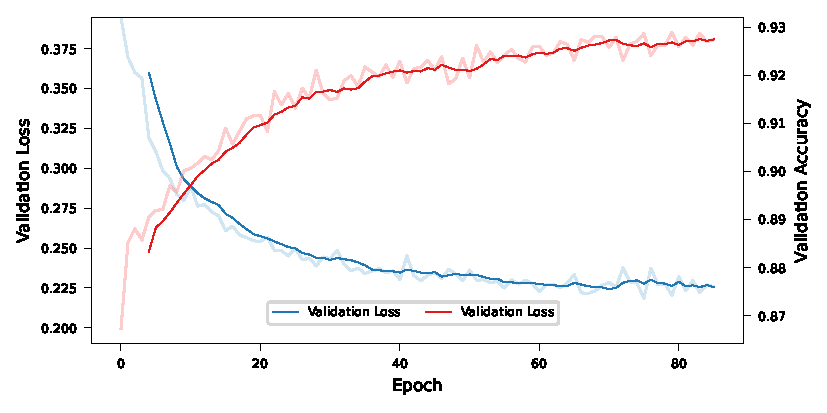
\includegraphics{figures/best_model_training_metrics.pdf}
    \caption{Validation loss and accuracy for the best model.}
    \label{fig:best_model_training_metrics}
\end{figure}

The accuracy per class, shown in \autoref{fig:best_model_accuracy_per_category},
aligns with expectations. Classes like \texttt{Building}, \texttt{GreenAreas}, \texttt{RoadAsphalt}, \texttt{Forest},
and \texttt{MeadowPasture} are predicted with high accuracy. Conversely, classes where there is
very little data available, like \texttt{WaterBasin}, or classes where the data is more vague,
like \texttt{ConstructionSites}, are predicted with lower accuracy.

From the visual inspection of the predictions in \autoref{fig:best_model_visual},
it looks like the borders between the classes are difficult to predict. This can be
explained by the fact that the classes are not always very precise, which specifically
affects these areas. Another explanation could be the resolution of 10 cm,
which leads to pixels in reality consisting of multiple classes. This issue, referred to
as mixed pixels, could be part of the reason for the lower accuracy in the
border areas.

\subsection{Hyperparameter Tuning}

The hyperparameter tuning process was successful in finding the best hyperparameters
within the grid search. From \autoref{fig:hp_tuning_boxplot}, it can be seen that
lower values for the \texttt{learning\_rate} seem to work better and that
a higher regularization during training -- a higher value of \texttt{weight\_decay} -- leads to
better results. Very interesting is the fact that the benefit of the data augmentation
seems to correlate with more regularization during training.
The grid of evaluated hyperparameters was rather limited due to limited computational
resources and the remaining time. A more extensive search could potentially lead to
even better results. What might really be worth trying is testing even smaller
values of \texttt{learning\_rate}, higher values for \texttt{weight\_decay}, 
and using other options for data augmentation --
pixel- and channel-noise in different combinations.

\subsection{Comparing the Results to the GIS Approach}

Since the validation for the original studies was done for a different area in Rünenberg,
using a different dataset, it is hard to compare the results directly. Adding to that,
different land cover categories were used, as well as different resolutions. Overall, the
original studies achieved an accuracy of 0.9 to 1 for the more obvious classes like
\texttt{Buildings}, \texttt{SealedRoads}, \texttt{GreenAreas}, and \texttt{MeadowPastures}. 
For the more difficult classes, like \texttt{PathUnsealed} and \texttt{SealedObjects}, the
accuracy was lower as well. The results of this study -- as differently as they were created --
reach a similar range of accuracy.

\subsection{Prospects}

The results of this study show that the approach of using deep learning for perviousness
classification is promising. The results are in a similar range as the results of the
original study using a GIS approach. Therefore, it might be worth further investigating
the potential of deep learning for this task. The next steps, besides the mentioned hyperparameter
expansion, more data augmentation, and more thorough training by going for more epochs, include other
promising approaches. One could be to try different model concepts like U-Net -- specifically
designed for image segmentation tasks. Another approach could be to use a pre-trained model
to build upon -- the issue there is finding a model that is trained on similar data and
accepts four channels as input. Another idea could be to implement some self-supervised
learning techniques utilizing unlabeled data to improve the model. As with most deep
learning tasks, the more data, the better -- so it would be worth trying to get more data
of possibly even higher quality to improve the existing models.
